\documentclass[10pt,a4paper]{article}
% EPTC 2026 -- main manuscript; pdfLaTeX + BibTeX, compatible with Overleaf.
\usepackage[margin=18mm,top=18mm,bottom=19mm]{geometry}
\usepackage[T1]{fontenc}
\usepackage[utf8]{inputenc}
\usepackage{lmodern,microtype}
\usepackage{amsmath,amssymb}
\usepackage{booktabs,tabularx,array}
\usepackage{graphicx}
\usepackage[dvipsnames]{xcolor}
\usepackage{tikz}
\usepackage{pgfplots}
\pgfplotsset{compat=1.17}
\usepackage{caption}
\usepackage{placeins} % Keep explanatory prose and its floats in reading order
\usepackage{enumitem}
\usepackage{natbib}
\usepackage{titlesec}
\usepackage{fancyhdr}
\usepackage{hyperref}
\hypersetup{colorlinks=true,linkcolor=NavyBlue,citecolor=NavyBlue,urlcolor=NavyBlue}
\definecolor{ink}{HTML}{153147}
\definecolor{midblue}{HTML}{34759B}
\definecolor{pale}{HTML}{EDF3F7}
\definecolor{steel}{HTML}{697987}
\definecolor{heat}{HTML}{DCE9F2}
\setlength{\parindent}{0pt}
\setlength{\parskip}{3pt}
\renewcommand{\baselinestretch}{1.02}
\setlist[itemize]{leftmargin=*,topsep=2pt,itemsep=1pt,parsep=0pt}
\titleformat{\section}{\large\bfseries\color{ink}}{\thesection}{0.55em}{}
\titleformat{\subsection}{\normalsize\bfseries\color{ink}}{\thesubsection}{0.55em}{}
\titlespacing*{\section}{0pt}{9pt}{3pt}
\titlespacing*{\subsection}{0pt}{6pt}{2pt}
\titleformat{\subsubsection}{\small\bfseries\color{ink}}{\thesubsubsection}{0.55em}{}
\titlespacing*{\subsubsection}{0pt}{5pt}{2pt}
\captionsetup{font=small,labelfont=bf,skip=3pt}
\pagestyle{fancy}
\fancyhf{}
\fancyhead[L]{\scriptsize EPTC 2026 | TIM1 co-design}
\fancyhead[R]{\scriptsize Representative 700-W FCBGA | thermal--mechanical analysis}
\fancyfoot[C]{\scriptsize \thepage}
\renewcommand{\headrulewidth}{0.25pt}
\setlength{\headheight}{13pt}
\newcommand{\Tmax}{T_{\mathrm{max}}}
\newcommand{\Reff}{R_{\mathrm{eff}}}
\newcommand{\BLT}{\mathrm{BLT}}
\newcommand{\kperp}{k_{\perp}}
\newcolumntype{Y}{>{\raggedright\arraybackslash}X}

\begin{document}
\begin{titlepage}
\thispagestyle{empty}
\vspace*{14mm}
{\small\bfseries\color{midblue} EPTC 2026 STUDENT INNOVATION CHALLENGE}\par
\vspace{4mm}
{\color{midblue}\rule{\linewidth}{1.4pt}}\par
\vspace{14mm}
{\Huge\bfseries\color{ink} Interface-Aware\\[3mm] Thermomechanical\\[3mm] Co-Design of TIM1}\par
\vspace{7mm}
{\Large for a Representative 700-W AI Accelerator FCBGA Package}\par
\vspace{12mm}
{\color{steel}\rule{0.28\linewidth}{0.7pt}}\par
\vspace{9mm}
{\large\bfseries Final Technical Report}\par
{\normalsize\color{steel} Thermal Interface Material Optimization for Advanced Electronics Packaging and Reliability}\par
\vspace{17mm}
\begin{tabularx}{\linewidth}{@{}p{35mm}Y@{}}
\textbf{Institution} & National University of Singapore (NUS)\\[3mm]
\textbf{Team members} & Fang Tianchi, Ke Tangxin, Du Yanzhang and Duan Yihe\\[3mm]
\textbf{Registered team} & \textcolor{BrickRed}{\textbf{[INSERT REGISTERED TEAM NAME]}}\\[3mm]
\textbf{EPTC Team ID} & \textcolor{BrickRed}{\textbf{[INSERT TEAM ID]}}\\
\end{tabularx}
\vfill
\noindent\colorbox{pale}{\parbox{\dimexpr\linewidth-2\fboxsep\relax}{
\small\textbf{Study scope.} Analytical checks, steady-state Icepak thermal screening,
contact-retention sensitivity, and matched one-way MAPDL structural analysis.
The paper compares simulated design alternatives; it does not claim measured hardware
performance, fatigue life or industrial qualification.}}
\vspace{6mm}
{\small\color{steel} Singapore \hfill 26 October 2026}
\end{titlepage}
\setcounter{page}{2}

\section*{Abstract}
\noindent\colorbox{pale}{\parbox{\dimexpr\linewidth-2\fboxsep\relax}{\small
A representative 700-W lidded flip-chip ball-grid-array (FCBGA) package was used
to investigate thermal-interface-material 1 (TIM1) conductivity, bond-line thickness
(BLT), retained contact area and simplified package mechanics. The approach combines
analytical resistance checks, numerical replication, a three-material thermal screen,
idealized contact-loss scenarios, nine carbon conductivity--BLT thermal solutions
and nine matched one-way thermomechanical analyses. Under ideal thermal contact,
grease, carbon-fiber and indium reference cases yielded peak die temperatures of
102.534, 93.344 and 81.883\,\textdegree C, respectively. At fixed carbon
$k_\perp=30$\,W/(m\,K), reducing BLT from 0.25 to 0.10\,mm lowered
peak temperature by 7.571\,\textdegree C and modeled lid warpage by 2.47\%,
but increased volume-averaged TIM stress by 9.46\% and mean elastic strain
by 10.86\%. Equal 64.82\% retained-contact fractions yielded highly different
thermal outcomes when missing-contact topology was varied. We recommend two
\emph{sampled} candidates: a 100-$\mu$m thermal-priority configuration
and a 250-$\mu$m lower-stress configuration, both at $k_\perp=30$\,W/(m\,K).
The results define a bounded engineering trade-off, not a universal optimum,
validated failure threshold or qualified manufactured material.}}\par
\vspace{2mm}
{\footnotesize\textbf{Keywords:} FCBGA; TIM1; carbon-fiber thermal pad; bond-line thickness;
interface coverage; warpage; thermomechanical FEA.}

\section{Problem Statement}
The heat-removal path of a high-power lidded package depends not only on bulk TIM conductivity but also
on compressed thickness, thermal contact resistance, conformity, pressure and aging
\citep{prasher2006,due2013,zhao2019}. Vertically oriented carbon-fiber TIMs can offer high through-plane
conductivity with useful compliance \citep{li2023,yi2025}; metallic indium is an instructive alternative,
with different bonding and constitutive-mechanics constraints \citep{wen2026}.
The characterization of compliant TIM mechanical properties is itself challenging \citep{subramanian2019};
recent studies emphasize coverage degradation and package-warpage-driven interface effects
\citep{du2026,yenigun2026}.
The question is how these properties and \emph{where} contact is retained jointly shape thermal and mechanical behavior.
The study follows a decision-oriented workflow: first establish a verified thermal reference, then examine how
contact area and contact \emph{location} affect heat removal, then compare conductivity and thickness
systematically, and finally evaluate the resulting structural response. The experimental variables are
through-plane conductivity, installed BLT, and idealized contact geometry. Mechanical sensitivity is evaluated
through several assumed \emph{effective} modulus/thermal-expansion combinations; these are not
measured material formulations. Thermal void studies and fully bonded mechanics are distinct scenarios:
we do not simulate progressive delamination, fatigue or pressure-dependent contact feedback.

The engineering contribution is a \emph{bounded comparison} that separates literature evidence,
simulation outputs and unverified material/assembly assumptions. This distinction matters because
a visually attractive low-temperature solution is not necessarily feasible as a compressed TIM layer.
Similarly, reduced global lid warpage does not guarantee lower local interfacial stress
\citep{subramanian2019,yenigun2026}.


\subsection{Design objectives and evaluation criteria}
A thermal-only screening exercise favors lower modeled peak die temperature. A package-level choice must
add mechanically relevant measures, here the volume-averaged TIM1 von Mises stress and equivalent elastic strain,
alongside lid-top warpage. These metrics are kept separate: a lower warpage result does not imply a lower
average TIM stress, and neither directly yields a fatigue life. For fair conductivity--thickness comparisons,
the same 700-W heat map, cooler boundary, TIM2 and package surroundings are retained.
For mechanical comparisons, the same representative property model is used at each thermal DOE point,
so an apparent conductivity effect is not confounded by switching modulus assumptions.
This design-of-experiments approach is supported by the broader TIM literature but the numerical cases
and their outputs belong to this study, not to the cited authors \citep{prasher2006,subramanian2019}.

\section{Methodology}
\subsection{Geometry, hotspot distribution and source traceability}
Figure~\ref{fig:model} illustrates the modeled heat path and prescribed 4$\times$4 hotspot distribution.
This is a \emph{representative test vehicle}, not an H100 floorplan or measured proprietary GPU.
The 16 tiles sum to $4(84)+8(42)+4(7)=700$\,W. Literature motivates the packaging form,
but study-defined quantities remain explicitly distinguished in Table~\ref{tab:provenance}.

\begin{figure}[htbp]
\centering
\begin{minipage}[c]{0.55\linewidth}\centering
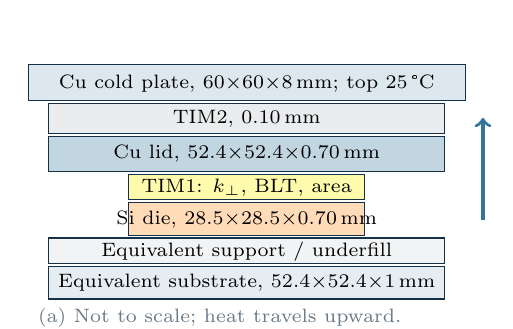
\begin{tikzpicture}[x=0.75cm,y=0.62cm,every node/.style={font=\scriptsize}]
\draw[fill=midblue!17,draw=ink] (0,6.0) rectangle (7.4,6.75);
\node at (3.7,6.36) {Cu cold plate, 60$\times$60$\times$8\,mm; top 25\,\textdegree C};
\draw[fill=steel!14,draw=ink] (0.35,5.33) rectangle (7.05,5.95);
\node at (3.7,5.64) {TIM2, 0.10\,mm};
\draw[fill=midblue!30,draw=ink] (0.35,4.55) rectangle (7.05,5.27);
\node at (3.7,4.91) {Cu lid, 52.4$\times$52.4$\times$0.70\,mm};
\draw[fill=yellow!32,draw=ink] (1.70,3.97) rectangle (5.70,4.49);
\node at (3.70,4.23) {TIM1: $\kperp$, BLT, area};
\draw[fill=orange!28,draw=ink] (1.70,3.24) rectangle (5.70,3.91);
\node at (3.70,3.57) {Si die, 28.5$\times$28.5$\times$0.70\,mm};
\draw[fill=steel!9,draw=ink] (0.35,2.66) rectangle (7.05,3.19);
\node at (3.7,2.92) {Equivalent support / underfill};
\draw[fill=midblue!13,draw=ink] (0.35,1.94) rectangle (7.05,2.61);
\node at (3.7,2.27) {Equivalent substrate, 52.4$\times$52.4$\times$1\,mm};
\node[anchor=west,text=steel] at (0,1.55) {(a) Not to scale; heat travels upward.};
\draw[->,very thick,midblue] (7.70,3.55) -- (7.70,5.65);
\end{tikzpicture}
\end{minipage}\hfill
\begin{minipage}[c]{0.41\linewidth}\centering
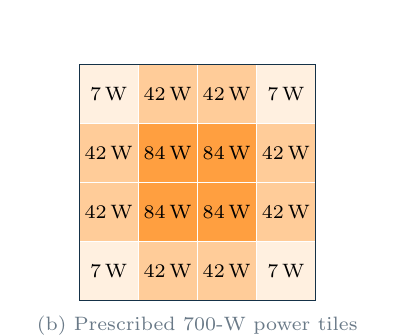
\begin{tikzpicture}[x=0.75cm,y=0.75cm]
\foreach \r/\c/\v/\sh in {
0/0/7/12,0/1/42/40,0/2/42/40,0/3/7/12,
1/0/42/40,1/1/84/75,1/2/84/75,1/3/42/40,
2/0/42/40,2/1/84/75,2/2/84/75,2/3/42/40,
3/0/7/12,3/1/42/40,3/2/42/40,3/3/7/12}
{\filldraw[fill=orange!\sh,draw=white,thin] (\c,3-\r) rectangle ++(1,1);
\node[font=\scriptsize] at (\c+0.5,3.5-\r) {\v\,W};}
\draw[draw=ink] (0,0) rectangle (4,4);
\node[font=\scriptsize,text=steel] at (2,-0.42) {(b) Prescribed 700-W power tiles};
\end{tikzpicture}
\end{minipage}
\caption{Constructed layer stack and study-defined hotspot pattern; diagrams are schematic rather than measured product geometry.}
\label{fig:model}
\end{figure}

\begin{table}[htbp]\centering
\caption{Dimensions, physical inputs and provenance; literature alignment does \emph{not} imply identical product geometry.}
\label{tab:provenance}
\footnotesize
\begin{tabularx}{\linewidth}{@{}p{30mm}p{67mm}Y@{}}
\toprule
Model item & Input & Evidence classification\\\midrule
Silicon die & $28.5\times28.5\times0.70$\,mm; $k=180$\,W/(m\,K) & Lateral area study-fixed; thickness/conductivity literature-aligned\\
TIM1 & $28.5\times28.5$\,mm; $k$ and BLT varied & Geometry and DOE study-defined; $k=21$ carbon anchor from \citet{yi2025}\\
Copper lid & $52.4\times52.4\times0.70$\,mm; $k=400$\,W/(m\,K) & Model aligned with \citet{wen2026}\\
TIM2 & $52.4\times52.4\times0.10$\,mm; $k=5.4$\,W/(m\,K) & Model aligned with \citet{wen2026}\\
Cold plate & $60\times60\times8$\,mm; upper surface 25\,\textdegree C & Footprint literature-aligned; thickness and boundary study-defined\\
Equivalent substrate & $52.4\times52.4\times1.0$\,mm & Geometry aligned with \citet{wen2026}; homogenized model\\
Die power & 700\,W over 16 imposed 84/42/7\,W tiles & Study-defined; not a measured accelerator floorplan\\
Carbon mechanics & $E=0.5/1/1.5$\,MPa; CTE $=250/180/100$\,ppm/K & Hypothetical linked SOFT/MID/STIFF brackets\\
\bottomrule
\end{tabularx}
\end{table}
\FloatBarrier

\subsection{Steady-state thermal model and mechanical handoff}
Steady-state thermal fields were obtained with Ansys AEDT/Icepak 2026 R1 under a fixed 25\,\textdegree C
cold-plate top boundary; cooling-fluid flow was not resolved.
MAPDL Classic quarter-symmetry SOLID186 mechanical analyses received \emph{reduced} thermal fields
(die-class and layer-average temperatures) from the corresponding Icepak cases.
The transfer is one-way, with fully bonded mechanical interfaces and no evolving gap/contact law.

For area $A=(28.5\,\mathrm{mm})^2$ we distinguish the bulk TIM metric and a modeled system metric:
\begin{equation}
 R_{\mathrm{bulk,TIM1}}=\frac{\BLT}{\kperp A},\qquad
 \Reff=\frac{T_{\mathrm{max,die}}-25\,^{\circ}\mathrm C}{700\,\mathrm W}.
 \label{eq:resistance}
\end{equation}
$\Reff$ is a \emph{peak-die-to-fixed-boundary} metric, not measured JEDEC $\theta_{JC}$
and not an intrinsic material property.

Mesh refinement of the grease reference changed peak temperature by 0.256\% and $\Reff$ by 0.339\%;
an independently rebuilt carbon reference agreed within 0.004\,\textdegree C.
The $k=21$\,W/(m\,K), 0.25-mm control in the conductivity--BLT study
reproduced the reference to within 0.000031\,\textdegree C.
These are numerical consistency tests, not experimental calibration.

An \emph{independent 45-W thermal-resistance diagnostic} fitted a study-selected
0.200\,\textdegree C/W package target from a modeled 0.14457\,\textdegree C/W
using an effective 8.65\,\textdegree C\,mm$^2$/W package-level penalty.
The fitted term was neither measured intrinsic TIM contact resistance nor applied
to the later 700-W simulations. The full-contact results are therefore best interpreted
as ideal-interface comparisons, not as unconditional predictions of actual assembled packages. Contact
resistance depends on roughness, pressure and interface temperature \citep{zhao2019}.


\subsection{Physical basis of the thermal comparison}
For a nominally uniform layer, the through-plane bulk resistance varies as BLT divided by
conductivity and area, as expressed in Eq.~\eqref{eq:resistance}. A real mounted interface has additional
thermal contact terms that may depend on pressure and surface condition:
\begin{equation}
R_{\mathrm{TIM1,installed}}\approx R_{\mathrm{contact,die}}+
\frac{\BLT}{\kperp A_{\mathrm{effective}}}
+R_{\mathrm{contact,lid}}.
\label{eq:contact}
\end{equation}
Equation~\eqref{eq:contact} is a useful physical interpretation rather than an additional fitted law
or a constitutive model solved in this project \citep{prasher2006,zhao2019,li2023}.
If contact is missing preferentially beneath a hotspot, the relevant \emph{spatial} heat path changes;
the total retained fraction by itself does not determine the peak die temperature.
A one-dimensional resistance term also does not capture lateral spreading through
the die and lid. Therefore, the modeled $\Reff$ is used for comparison of \emph{whole-package}
thermal responses rather than being identified with TIM1 bulk or interfacial resistance.

\section{Results and Analysis}
\subsection{Grease, carbon-fiber and indium reference comparison}
\begin{table}[htbp]\centering
\caption{Material-family references at 700\,W with ideally retained TIM1 area; BLTs also differ.}
\label{tab:materials}
\small
\begin{tabular}{@{}lrrrr@{}}\toprule
TIM1 & $k_{\perp}$ [W/(m\,K)] & BLT [mm] & $\Tmax$ [\textdegree C] & $\Reff$ [\textdegree C/W]\\\midrule
Grease & 5 & 0.09 & 102.534 & 0.110762\\
Carbon fiber & 21 & 0.25 & 93.344 & 0.097634\\
Indium & 86 & 0.40 & 81.883 & 0.081262\\\bottomrule
\end{tabular}
\end{table}
Relative to the grease reference, carbon lowers the simulated peak temperature by 9.19\,\textdegree C
and indium by 20.65\,\textdegree C. These are \emph{material-and-BLT} comparisons, not a
single-variable conductivity or durability ranking.
An assumed compliant-grease mechanics case ($E=0.05$\,MPa) produced 0.00105\,MPa mean TIM stress and
15.51\,$\mu$m lid warpage. A purely elastic indium run yielded 50.90\,MPa mean stress, not a defensible
post-yield service prediction; assumed 1.00/2.14\,MPa-yield bilinear cases instead gave about
0.51/0.49\% mean plastic strain. Single-load simulations cannot rank fatigue life.

\subsection{Influence of retained contact area and its spatial distribution}
\citet{yi2025} measured carbon-pad retained coverage of 88.22\% after packaging
and 64.82\% after subsequent preconditioning/reliability exposure.
We apply these \emph{area fractions}, not their measured acoustic-microscopy shapes,
to designed idealized missing-TIM geometries.
For the reference $k=21$\,W/(m\,K), BLT=0.25\,mm,
100\% coverage yielded 93.344\,\textdegree C,
a centered 88.22\% footprint 93.653\,\textdegree C,
and a centered 64.82\% footprint 109.758\,\textdegree C.

\begin{table}[htbp]\centering
\caption{Three \emph{assumed} spatial loss patterns at the same 64.82\% retained TIM area. Tile indices start at one.}
\label{tab:topology}
\small
\begin{tabular}{@{}lrrl@{}}\toprule
Loss pattern & $\Tmax$ [\textdegree C] & $\Reff$ [\textdegree C/W] & Hottest tile (row,col)\\\midrule
Peripheral ring loss & 109.758 & 0.121083 & (2,1)\\
One missing edge band & 417.839 & 0.561198 & (1,2)\\
Central square void & 400.546 & 0.536495 & (3,3)\\\bottomrule
\end{tabular}
\end{table}

\begin{figure}[htbp]
\centering
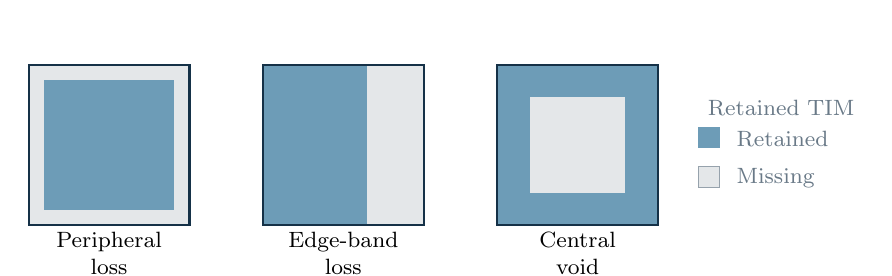
\begin{tikzpicture}[x=0.85cm,y=0.85cm]
% Full square denotes die footprint. Dark region is retained TIM1, light region is missing TIM1.
\begin{scope}[shift={(0,0)}]
 \fill[steel!18] (0,0) rectangle (2.4,2.4);
 \fill[midblue!72] (0.232,0.232) rectangle (2.168,2.168);
 \draw[ink,thick] (0,0) rectangle (2.4,2.4);
 \node[font=\footnotesize,align=center] at (1.2,-0.42) {Peripheral\\loss};
\end{scope}
\begin{scope}[shift={(3.5,0)}]
 \fill[steel!18] (0,0) rectangle (2.4,2.4);
 \fill[midblue!72] (0,0) rectangle (1.556,2.4);
 \draw[ink,thick] (0,0) rectangle (2.4,2.4);
 \node[font=\footnotesize,align=center] at (1.2,-0.42) {Edge-band\\loss};
\end{scope}
\begin{scope}[shift={(7,0)}]
 \fill[midblue!72] (0,0) rectangle (2.4,2.4);
 \fill[steel!18] (0.488,0.488) rectangle (1.912,1.912);
 \draw[ink,thick] (0,0) rectangle (2.4,2.4);
 \node[font=\footnotesize,align=center] at (1.2,-0.42) {Central\\void};
\end{scope}
\node[anchor=west,font=\footnotesize,text=steel] at (10.0,1.75) {Retained TIM};
\fill[midblue!72] (10.0,1.15) rectangle (10.32,1.47);
\node[anchor=west,font=\footnotesize,text=steel] at (10.43,1.29) {Retained};
\fill[steel!18,draw=ink!45] (10.0,0.56) rectangle (10.32,0.88);
\node[anchor=west,font=\footnotesize,text=steel] at (10.43,0.70) {Missing};
\end{tikzpicture}
\caption{Illustrative \emph{assumed} contact-loss topologies at approximately the same
64.82\% retained area. The dark regions depict remaining TIM1, not measured acoustic images;
the drawings clarify topology rather than claiming exact simulated meshing.}
\label{fig:topology}
\end{figure}
\FloatBarrier

At equal retained area, the \emph{location} of remaining conductive paths matters greatly.
The 400\,\textdegree C-class outputs are severe model-specific conductive-blockage scenarios:
they are not measured aging temperatures, operating thresholds, or physically validated predictions.
These patterns lack independent topology-specific mesh and experiment-based verification
and neglect calibrated air-gap and pressure-dependent transport.

These differences should not be misread as a prediction that all packages with 64.82\% contact
will reach similarly high temperatures. The model applies idealized severe blockage at selected places;
an actual interfacial gap may still transmit heat through trapped gas, residual material, or partial contact.
The comparison instead demonstrates a limitation of an \emph{area-only} TIM specification:
two interfaces with equal percent coverage need not have equal peak thermal resistance.
Published reports of packaging-induced area loss \citep{yi2025} and coupled warpage/interface behavior
\citep{du2026,yenigun2026} motivate measuring where contact is retained, not just how much.


\subsection{Thermal optimization across conductivity and bond-line thickness}
\subsubsection{Nine-case full-contact thermal design of experiments}
The factorial DOE varies $\kperp=\{15,21,30\}$\,W/(m\,K)
and $\BLT=\{0.10,0.25,0.40\}$\,mm while fixing the remaining study conditions.
\begin{table}[htbp]\centering
\caption{Solved peak die temperatures [\textdegree C] for the nine full-contact conductivity--thickness combinations.}
\label{tab:v4b}
\small
\begin{tabular}{@{}lrrr@{}}\toprule
$k$ [W/(m\,K)] & BLT 100\,$\mu$m & BLT 250\,$\mu$m & BLT 400\,$\mu$m\\\midrule
15 & 85.490 & 100.323 & 114.389\\
21 & 82.625 & 93.344 & 103.544\\
30 & \textbf{80.455} & 88.026 & 95.194\\\bottomrule
\end{tabular}
\end{table}

\begin{figure}[htbp]\centering
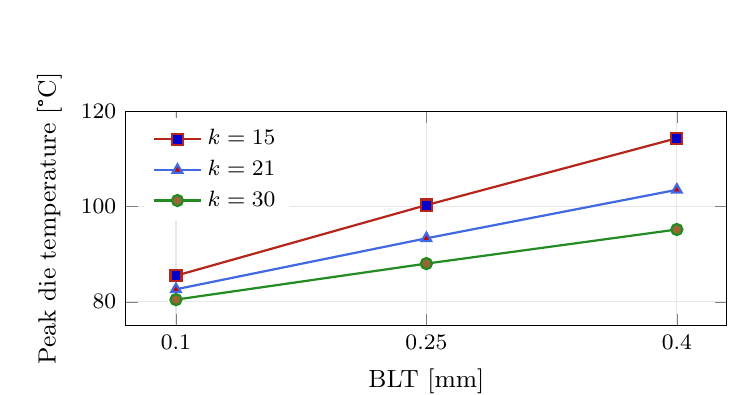
\begin{tikzpicture}
\begin{axis}[width=0.76\linewidth,height=43mm,xlabel={BLT [mm]},ylabel={Peak die temperature [\textdegree C]},
xmin=0.07,xmax=0.43,ymin=75,ymax=120,xtick={0.1,0.25,0.4},
grid=major,grid style={draw=black!9},legend pos=north west,
legend style={font=\footnotesize,draw=none},tick label style={font=\footnotesize},
label style={font=\small}]
\addplot+[mark=square*,thick,color=BrickRed] coordinates {(0.10,85.490)(0.25,100.323)(0.40,114.389)};
\addlegendentry{$k=15$}
\addplot+[mark=triangle*,thick,color=RoyalBlue] coordinates {(0.10,82.625)(0.25,93.344)(0.40,103.544)};
\addlegendentry{$k=21$}
\addplot+[mark=*,thick,color=ForestGreen] coordinates {(0.10,80.455)(0.25,88.026)(0.40,95.194)};
\addlegendentry{$k=30$}
\end{axis}
\end{tikzpicture}
\caption{Discrete conductivity--thickness thermal response. Lines connect sampled cases; continuous global optimality is not established.}
\label{fig:thermal}
\end{figure}
\FloatBarrier
At $k=21$, 250$\rightarrow$100\,$\mu$m improves $\Tmax$ by 10.719\,\textdegree C.
At BLT 250\,$\mu$m, $k=21\rightarrow30$ lowers $\Tmax$ by 5.318\,\textdegree C.
The lowest \emph{sampled} clean temperature is 80.455\,\textdegree C,
$\Reff=0.079221$\,\textdegree C/W, at $k=30$ and 100\,$\mu$m;
this is a targeted, not experimentally qualified, material and assembly state.


\subsubsection{Interpreting the conductivity--thickness trend}
The DOE distinguishes two decisions that are often conflated. At a \emph{fixed} conductivity,
a reduction in installed BLT shortens the bulk conduction path. At a \emph{fixed} thickness,
increasing through-plane conductivity has a similar direction of thermal benefit, but not
necessarily the same quantitative leverage. Their combined effect must still be evaluated
with the nonuniform heat source and package conduction paths.
The $k=30$\,W/(m\,K), 100-$\mu$m configuration is thus a \emph{modeled target}; it should
not be described as an off-the-shelf carbon material that was physically fabricated or
thermally tested. Research on aligned carbon-fiber networks supports the feasibility of
high conductivity and tunable compliance as \emph{material concepts}, but does not
validate the modulus, compressed thickness or adhesion assumed here
\citep{li2023,yi2025,subramanian2019}.

\subsubsection{Independent confirmation under partial contact retention}
\begin{table}[htbp]\centering
\caption{Four independently checked thermal configurations at full or 88.22\% retained TIM1 contact area.}
\label{tab:v4c}
\small
\begin{tabular}{@{}lrrrr@{}}\toprule
Configuration & $k$ & BLT [mm] & Retained area & $\Tmax$ [\textdegree C]\\\midrule
Reference full & 21 & 0.25 & 100\% & 93.344\\
Reference retained & 21 & 0.25 & 88.22\% & 93.653\\
High-$k$ retained & 30 & 0.25 & 88.22\% & 88.295\\
Thin/high-$k$ retained & 30 & 0.10 & 88.22\% & \textbf{80.650}\\\bottomrule
\end{tabular}
\end{table}
An initially interrupted thin/high-conductivity solver run was recovered without changing
the model inputs. Only the subsequently completed four-case result set is used here.
The last case has $\Reff=0.0794998$\,\textdegree C/W.
Relative to the full-coverage $k=21$, 250-$\mu$m reference it is 12.694\,\textdegree C cooler;
because $k$, BLT and contact conditions differ, this is not a single-variable causal effect.

\subsection{Thermomechanical sensitivity and matched comparison}
\subsubsection{Effective material-property sensitivity and mesh verification}
An initial structural sensitivity comparison paired two \emph{different thermal} designs:
$k=21$\,W/(m\,K), BLT 250\,$\mu$m and $k=30$\,W/(m\,K), BLT 100\,$\mu$m.
Three hypothetical effective-property combinations were used: low modulus ($E=0.5$\,MPa,
CTE=250\,ppm/K), reference modulus ($E=1.0$\,MPa, CTE=180\,ppm/K),
and higher modulus ($E=1.5$\,MPa, CTE=100\,ppm/K),
with $\nu=0.49$ in all cases. $E$ and CTE change \emph{together}; these are not separately
identified properties nor measured constitutive fits.

\begin{table}[htbp]\centering
\caption{Fully bonded mechanical sensitivity. Stress and equivalent elastic strain are TIM1 volume-average quantities.}
\label{tab:v4d}
\small
\begin{tabular}{@{}lrrrr@{}}\toprule
Bracket / design & BLT [mm] & Mean VM [MPa] & Mean strain [\%] & Warpage [$\mu$m]\\\midrule
Low modulus ($k=21$) & 0.25 & 0.007812 & 1.595 & 17.380\\
Low modulus ($k=30$) & 0.10 & 0.007622 & 1.586 & 16.212\\
Reference ($k=21$) & 0.25 & 0.011339 & 1.159 & 19.012\\
Reference ($k=30$) & 0.10 & 0.011866 & 1.228 & 17.155\\
Higher modulus ($k=21$) & 0.25 & 0.010054 & 0.694 & 19.874\\
Higher modulus ($k=30$) & 0.10 & 0.012794 & 0.883 & 17.587\\\bottomrule
\end{tabular}
\end{table}
\FloatBarrier
The paired scenario reduced lid warpage by 6.72--11.51\% across property combinations,
while the higher-modulus case increased mean stress by 27.25\% and mean strain by 27.32\%.
For the 100-$\mu$m reference-modulus model, intermediate-to-fine mesh refinement changed
mean stress by +0.59\%, strain by $-1.96$\%, and warpage by $-0.038$\%.
However, \emph{local peak stress changed by about 50.2\%}. Accordingly, pointwise peak
stress is \textbf{not a converged failure metric}; only averaged mechanical trends and
warpage are emphasized. Furthermore, this original pair varied conductivity,
thickness \emph{and} the thermal loading simultaneously.
It could not isolate the source of the mechanical difference.
A common material model combined with all nine solved thermal conditions is needed
for a more interpretable design comparison.

\subsubsection{Matched nine-case thermal-to-mechanical analysis}
Every conductivity--thickness thermal configuration was coupled one-way to
the same \emph{reference-modulus} carbon mechanical model:
$E=1.0$\,MPa, CTE=180\,ppm/K, $\nu=0.49$.
Two previously solved matching configurations served as numerical reproduction checks.
The final comparison therefore contains nine solved thermal fields
and nine corresponding mechanical runs, rather than interpolated temperatures.
The thermal field is changed consistently with each design, while the nominal mechanical
property inputs remain fixed.


\subsubsection{What the matched design can and cannot isolate}
Using the same effective modulus, Poisson ratio and CTE across the nine mechanical simulations
removes the property-bracket confound in the initial two-design comparison. It does \emph{not}
hold the thermal field constant: temperature is a physical result of changing conductivity and
thickness and is intentionally transferred into the corresponding structural model.
Consequently, the stress differences represent a \emph{total design response} under a
specified one-way modeling protocol, rather than an isolated direct thickness effect at
identical temperature. This distinction is important when drawing mechanism-level conclusions.
Likewise, volume-averaged TIM stress is an engineering comparison metric, not a direct
delamination criterion: local adhesion, cohesive strengths and cyclic constitutive behavior
were not supplied \citep{subramanian2019,yenigun2026}.

\begin{table}[htbp]\centering
\caption{Matched nine-case thermal-to-mechanical results with one common reference-modulus material model.}
\label{tab:v6a}
\small
\begin{tabular}{@{}rrrrrr@{}}\toprule
$k$ [W/(m\,K)] & BLT [mm] & $\Tmax$ [\textdegree C] & Mean VM [MPa] & Mean strain [\%] & Warpage [$\mu$m]\\\midrule
15 & 0.10 & 85.490 & 0.012094 & 1.2568 & 18.611\\
15 & 0.25 & 100.323 & 0.012014 & 1.2296 & 20.948\\
15 & 0.40 & 114.389 & 0.013286 & 1.3535 & 23.503\\
21 & 0.10 & 82.625 & 0.011960 & 1.2400 & 17.778\\
21 & 0.25 & 93.344 & 0.011339 & 1.1594 & 19.012\\
21 & 0.40 & 103.544 & 0.012153 & 1.2369 & 20.496\\
30 & 0.10 & \textbf{80.455} & 0.011866 & 1.2279 & \textbf{17.155}\\
30 & 0.25 & 88.026 & \textbf{0.010841} & \textbf{1.1076} & 17.590\\
30 & 0.40 & 95.194 & 0.011306 & 1.1498 & 18.293\\\bottomrule
\end{tabular}
\end{table}
\begin{figure}[htbp]\centering
\begin{minipage}{0.49\linewidth}\centering
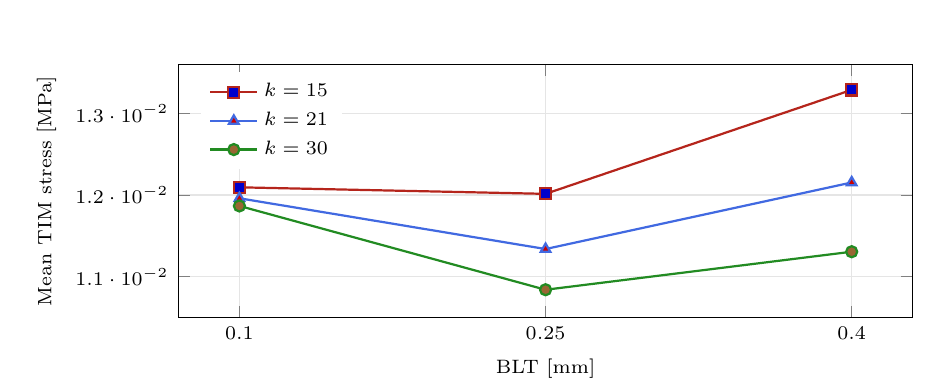
\begin{tikzpicture}
\begin{axis}[width=0.90\linewidth,height=48mm,xmin=0.07,xmax=0.43,ymin=0.0105,ymax=0.0136,
xtick={0.1,0.25,0.4},xlabel={BLT [mm]},ylabel={Mean TIM stress [MPa]},
grid=major,grid style={draw=black!10},scaled y ticks=false,
tick label style={font=\scriptsize},label style={font=\scriptsize},
legend style={font=\scriptsize,draw=none,at={(0.03,0.97)},anchor=north west}]
\addplot+[mark=square*,BrickRed,thick] coordinates {(0.1,0.012094)(0.25,0.012014)(0.4,0.013286)};
\addlegendentry{$k=15$}
\addplot+[mark=triangle*,RoyalBlue,thick] coordinates {(0.1,0.011960)(0.25,0.011339)(0.4,0.012153)};
\addlegendentry{$k=21$}
\addplot+[mark=*,ForestGreen,thick] coordinates {(0.1,0.011866)(0.25,0.010841)(0.4,0.011306)};
\addlegendentry{$k=30$}
\end{axis}
\end{tikzpicture}
\end{minipage}\hfill
\begin{minipage}{0.49\linewidth}\centering
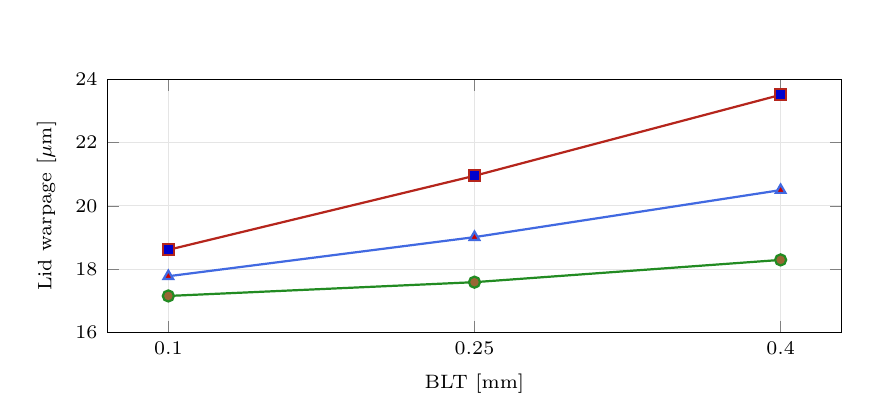
\begin{tikzpicture}
\begin{axis}[width=0.90\linewidth,height=48mm,xmin=0.07,xmax=0.43,ymin=16,ymax=24,
xtick={0.1,0.25,0.4},xlabel={BLT [mm]},ylabel={Lid warpage [$\mu$m]},
grid=major,grid style={draw=black!10},
tick label style={font=\scriptsize},label style={font=\scriptsize}]
\addplot+[mark=square*,BrickRed,thick] coordinates {(0.1,18.611)(0.25,20.948)(0.4,23.503)};
\addplot+[mark=triangle*,RoyalBlue,thick] coordinates {(0.1,17.778)(0.25,19.012)(0.4,20.496)};
\addplot+[mark=*,ForestGreen,thick] coordinates {(0.1,17.155)(0.25,17.590)(0.4,18.293)};
\end{axis}
\end{tikzpicture}
\end{minipage}
\caption{Matched structural response with fixed reference-modulus properties: the 250-$\mu$m sample minimizes
mean TIM stress at each sampled $k$, while thinner BLT favors temperature and modeled warpage.}
\label{fig:v6a}
\end{figure}
\FloatBarrier

At fixed $k=30$\,W/(m\,K), 250$\rightarrow$100\,$\mu$m reduces peak temperature
by 7.571\,\textdegree C and warpage by 2.47\%, but \emph{increases} mean stress
0.010841$\rightarrow$0.011866\,MPa (+9.46\%) and mean strain
1.1076$\rightarrow$1.2279\% (+10.86\%).
The 250-$\mu$m point gives the lowest mean stress and strain at \emph{each of the three sampled conductivities},
but this does not prove a continuous/global optimum.
Holding BLT at 250\,$\mu$m while increasing $k$ from 15 to 30
reduces peak temperature by 12.297\,\textdegree C and also lowers mean stress,
mean strain and warpage in the \emph{assumed reference-modulus model}.
The main observed mechanical compromise thus tracks BLT, not an inherent penalty from raising $k$.

\section{Discussion and Optimization}

\begin{figure}[htbp]\centering
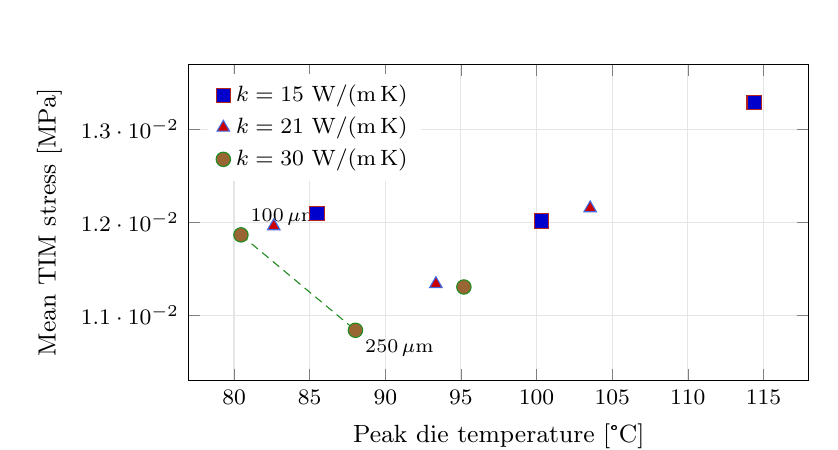
\begin{tikzpicture}
\begin{axis}[width=0.78\linewidth,height=56mm,
xlabel={Peak die temperature [\textdegree C]},ylabel={Mean TIM stress [MPa]},
xmin=77,xmax=118,ymin=0.0103,ymax=0.0137,
grid=major,grid style={draw=black!10},
legend pos=north west,legend style={draw=none,font=\footnotesize},
tick label style={font=\footnotesize},label style={font=\small},
scaled y ticks=false]
\addplot+[only marks,mark=square*,mark size=2.6pt,color=BrickRed]
 coordinates {(85.490,0.012094)(100.323,0.012014)(114.389,0.013286)};
\addlegendentry{$k=15$ W/(m\,K)}
\addplot+[only marks,mark=triangle*,mark size=2.6pt,color=RoyalBlue]
 coordinates {(82.625,0.011960)(93.344,0.011339)(103.544,0.012153)};
\addlegendentry{$k=21$ W/(m\,K)}
\addplot+[only marks,mark=*,mark size=2.6pt,color=ForestGreen]
 coordinates {(80.455,0.011866)(88.026,0.010841)(95.194,0.011306)};
\addlegendentry{$k=30$ W/(m\,K)}
\draw[densely dashed,ForestGreen] (axis cs:80.455,0.011866) -- (axis cs:88.026,0.010841);
\node[font=\scriptsize,anchor=south west,align=left] at (axis cs:80.455,0.011866)
 {100\,$\mu$m};
\node[font=\scriptsize,anchor=north west] at (axis cs:88.026,0.010841)
 {250\,$\mu$m};
\end{axis}
\end{tikzpicture}
\caption{Discrete modeled temperature--mean-stress trade-off.
The two labeled $k=30$\,W/(m\,K) points demonstrate the lower-temperature/higher-mean-stress
versus higher-temperature/lower-mean-stress choice. The dashed line is a guide, not a fitted response.}
\label{fig:tradeoff}
\end{figure}
\FloatBarrier

\begin{table}[htbp]\centering
\caption{Conditional carbon candidates, combining \emph{separate} clean/retained thermal scenarios with fully bonded reference-modulus mechanics.}
\label{tab:decision}
\footnotesize
\begin{tabularx}{\linewidth}{@{}p{37mm}rrrrY@{}}\toprule
Carbon configuration & Clean $\Tmax$ & 88.22\% $\Tmax$ & Mean VM & Warpage & Trade-off\\
 & [\textdegree C] & [\textdegree C] & [MPa] & [$\mu$m] & \\\midrule
\textbf{Thermal stretch}: $k=30$, BLT 100\,$\mu$m & \textbf{80.455} & \textbf{80.650} & 0.011866 & \textbf{17.155} & Best sampled thermal and warpage; higher mean stress/strain\\
\textbf{Lower-stress}: $k=30$, BLT 250\,$\mu$m & 88.026 & 88.295 & \textbf{0.010841} & 17.590 & Minimum sampled average TIM stress/strain\\
Reference: $k=21$, BLT 250\,$\mu$m & 93.344 & 93.653 & 0.011339 & 19.012 & Literature-anchored $k$ baseline\\\bottomrule
\end{tabularx}
\end{table}
\FloatBarrier

This is a \emph{multi-objective} selection rather than a ranking by one scalar.
A thermal-priority design favors the 100-$\mu$m case because both modeled peak temperature
and warpage are lower. A mechanical-load-priority design favors 250\,$\mu$m because
both averaged TIM stress and elastic strain are lower at fixed conductivity.
At all three conductivities sampled, 400\,$\mu$m is unattractive relative to
250\,$\mu$m in the combined simulated metrics: temperature, average stress/strain and warpage
are all higher. This conclusion is restricted to the three tested thickness levels.
The candidate comparison does not establish a yield, cost, lifetime or process-window optimum.
A material vendor may impose a minimum viable compressed BLT or a contact-pressure
requirement that changes which sampled point is physically achievable.

The 100-$\mu$m candidate targets lowest peak die temperature and modeled warpage where
compressed-pad feasibility and interface reliability can be demonstrated.
The 250-$\mu$m candidate accepts a 7.571\,\textdegree C higher clean temperature and
0.435\,$\mu$m more warpage at $k=30$ but minimizes sampled mean stress/strain.
These outputs do not predict relative service lifetime; moreover, the 30/250 candidate has
not been compared under the low- and higher-modulus sensitivity assumptions. The central design finding is
\[
\fbox{$\displaystyle\text{High } k \text{ helps broadly in this model; BLT creates the sampled thermal--mechanical trade-off.}$}
\]

\subsection{Model limitations and industrial qualification}
The 25\,\textdegree C isothermal cold-plate top is not resolved coolant flow, and the 700-W
pattern is not a measured commercial floorplan. Extreme topology cases are not measured
contact maps and lack independent topology-specific mesh validation. The thermal contact
penalty calibrated at 45\,W was not applied to later nominally ideal interfaces. Carbon
mechanics are assumed isotropic low-/reference-/higher-modulus property combinations, not measured
temperature-dependent properties of a manufactured $k=30$ carbon pad.
The quarter-package mechanics remain elastic, fully bonded and one-way/reduced-field;
no pressure-dependent contact resistance, cohesive failure, cycling, creep, pump-out,
plasticity in carbon, fatigue life or manufacturing yield was established.
\emph{Peak local stress was not mesh-converged and is not used as a failure criterion.}


\begin{table}[htbp]\centering
\caption{Evidence maturity and the highest-value measurements required before product qualification.}
\label{tab:maturity}
\footnotesize
\begin{tabularx}{\linewidth}{@{}p{31mm}p{53mm}Y@{}}
\toprule
Question & Supported in this study & Still required before claiming package reliability\\\midrule
Thermal comparison & Solved steady-state cases; mesh/reference replication checks & Measured boundary conditions, assembled temperature maps and compressed BLT\\
Contact retention & Fixed-area geometric sensitivity to idealized loss position & Observed spatial contact maps, pressure-dependent conductance, void/gas transport\\
Thermomechanics & Matched one-way reduced-field solutions, mean stress/strain and warpage & Temperature-dependent measured TIM laws, interfaces, cycling and fracture criteria\\
Design selection & Relative ranking among tested $k$--BLT combinations & Manufacturing capability, long-term adhesion and thermal-cycling statistics\\
\bottomrule
\end{tabularx}
\end{table}
\FloatBarrier

The next qualification path is to measure compressed BLT and anisotropic conductivity;
measure how contact resistance and adhesion vary with pressure and temperature;
map retained contact after warpage and cycling; and only then conduct
validated coupled simulations and package experiments.
Within its bounded assumptions, the study shows why TIM1 should be screened jointly
on thermal conductivity, installed thickness, spatial interface integrity and mechanical
accommodation---not on nominal $k$ or coverage percentage alone.


\section{Conclusion and Recommendations}
Three findings emerge from the same representative FCBGA model.
First, intrinsic conductivity cannot be ranked in isolation from installed thickness and
the quality of both contact surfaces. Second, the location of missing TIM1 contact
can change thermal behavior drastically even at a fixed retained area; extreme
blockage-model temperatures are \emph{not} reliability predictions.
Third, a matched nine-point thermal-to-mechanical study identifies a sampled
trade-off: the $k=30$\,W/(m\,K), 100-$\mu$m design has the best modeled
peak temperature and warpage, whereas the 250-$\mu$m alternative has the
smallest mean stress and strain. This result does not certify either design for service.
The actionable contribution is a reproducible method for making TIM1 choices
based on thermal and mechanical objectives \emph{together}, with explicit
source traceability and defined verification gaps.

{\small
\bibliographystyle{unsrtnat}
\bibliography{references}
}
\end{document}
